\label{Section: Introduction}
\section{Introduction}

\begin{frame}{Background}\label{Introduction: Development of ICSs}
    Driven by computer technology, communication technology and intellectual technology, Industrial Control Systems (ICSs) develop towards the direction of intellectualization and network.
    \begin{center}
        \begin{tikzpicture}[line width = \pgfdefaultlinewidth,
                    revolution/.style = {align = left, below = 4.5pt, right, font = \scriptsize}]

    \draw[->] (-0.4,0) -- (0,0) -- (10,0) node [anchor = north east] {Time};
    \draw[->] (0,-0.4) -- (0,0) -- (0,5.7) node [midway,sloped,above] {Degree of Automation};

    \coordinate (A) at (0.5, 0.5);
    \coordinate (B) at (2.5, 1.5);
    \coordinate (C) at (4.5, 3.0);
    \coordinate (D) at (6.5, 5.0);


    \fill (A) circle (2pt) node [revolution] {The 1\textsuperscript{st} industrial revolution\\Machine Age};
    \pause
    \fill (B) circle (2pt) node [revolution] {The 2\textsuperscript{nd} industrial revolution\\Semi-automatic Age};
    \pause
    \fill (C) circle (2pt) node [revolution] {The 3\textsuperscript{rd} industrial revolution\\Automatic Age};
    \pause
    \fill (D) circle (2pt) node [revolution] {The 4\textsuperscript{th} industrial revolution\\Intelligent Age};

    \pause
    \draw[postaction={decoration={text along path, transform={yshift=5pt}, text color=red, text={The Development of Industrial Control Systems},
text align=center}, decorate}]
    [domain=0.25:7, variable=\x, samples=200, ->, red, line width = 2pt] plot({\x},{(0.0625*\x^2 + 0.3125*\x + 0.3281)});
    
    
    
    
\end{tikzpicture} 
    \end{center}
\end{frame}

\begin{frame}{Background}\label{Introduction: ICSs are Important}
    \begin{itemize}
      \item ICSs have been widely applied in various industry of the national economy and people's livelihood, and gradually become the brain and central nervous of critical infrastructure and all kinds of industrial production.
      \item Once abnormal situation appears in ICSs , serious accidents may be happen, which may cause damage to property, people or a wide range of environment.
    \end{itemize}

    \begin{center}
      \begin{minipage}[m]{0.9\textwidth}
        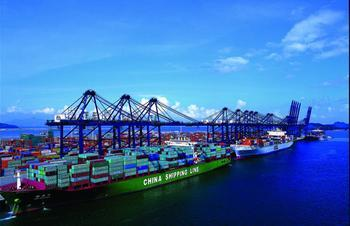
\includegraphics[height=1.5cm]{Figures/Introduction/Fig1.png} \hfill
        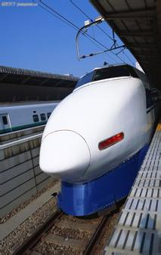
\includegraphics[height=1.5cm]{Figures/Introduction/Fig2.png} \hfill
        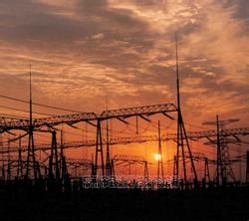
\includegraphics[height=1.5cm]{Figures/Introduction/Fig3.png} \hfill
        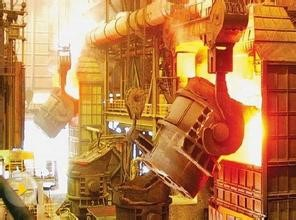
\includegraphics[height=1.5cm]{Figures/Introduction/Fig4.png} \hfill
        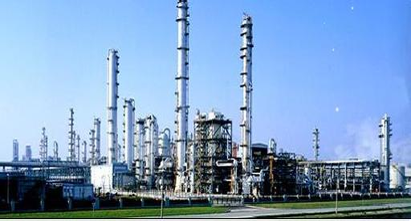
\includegraphics[height=1.5cm]{Figures/Introduction/Fig5.png} \vspace{1pt}\\
        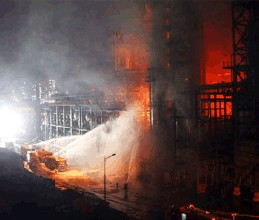
\includegraphics[height=1.5cm, width = 2.2cm]{Figures/Introduction/Fig6.png} \hfill
        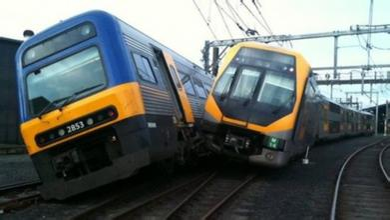
\includegraphics[height=1.5cm]{Figures/Introduction/Fig7.png} \hfill
        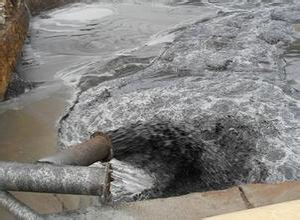
\includegraphics[height=1.5cm]{Figures/Introduction/Fig8.png} \hfill
        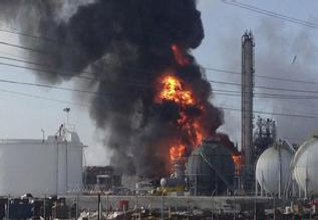
\includegraphics[height=1.5cm]{Figures/Introduction/Fig9.png}
      \end{minipage}
    \end{center}
\end{frame}

\begin{frame}{Background}\label{Introduction: ICSs are under Attacks}
    \begin{itemize}
      \item In 2010, Stuxnet attacked Iran's nuclear power plants and ruined almost one-fifth of Iran's nuclear centrifuges.
      \item In 2013, Israel Haifa highway control system  was attacked by hackers, which caused massive traffic congestion in the city which lead great loss and serious subsequent problems.
      \item In 2014, Havex malware infects many industrial control system in European  and caused the leakage of large amounts of data.
    \end{itemize}

    \begin{minipage}[c][][t]{0.6\textwidth}
      \begin{tikzpicture}[line width = \pgfdefaultlinewidth]

    \begin{axis}[symbolic x coords={2010, 2011, 2012, 2013, 2014},
                 xtick=data,
                 xlabel = {\footnotesize ICSs Event Statistic (ICS-CERT)},
                 width = 7cm,
                 height = 4.5cm,
                 nodes near coords,
                 ymax = 300,
                 ymin = 0]
        \addplot[ybar,fill=black] coordinates {
            (2010,39)
            (2011,140)
            (2012,197)
            (2013,257)
            (2014,245)
    };
\end{axis}
\end{tikzpicture} 
    \end{minipage}
    \begin{minipage}[c][][t]{0.35\textwidth}
    \begin{tikzpicture}
      \node (A) at (0,1.5) {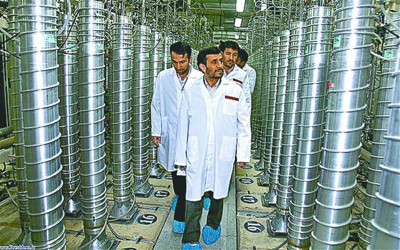
\includegraphics[height=2.2cm]{Figures/Introduction/Fig10.png}};
      \node[line width = 3pt, draw = white, inner sep=0pt] (B) at (1,0) {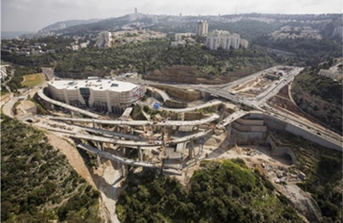
\includegraphics[height=2.2cm]{Figures/Introduction/Fig11.png}};
    \end{tikzpicture}
    \end{minipage}
\end{frame}

\begin{frame}{Problems -- Timeliness and Availability}\label{Introduction: Problem of Timeliness and Availability}
    ICSs have rigorous requirements on timeliness and availability. The cybersecurity risks of ICSs are primarily from the potential loss caused by the cyber-attacks which demolish the timeliness and availability of the control system.
    
    \pause
    In order to achieve the destructive purpose, attackers generally need to follow part or all of these three steps:
    \begin{enumerate}
      \item infiltrate into the field network,
      \item invalidate the system functions,
      \item cause the hazardous incidents.
    \end{enumerate}

    \pause
    Therefore, the cybersecurity risk assessment of ICSs needs  a novel and targeted risk model to analyze the risk propagation.
\end{frame}

\begin{frame}{Problems -- Overlapping amongst Consequences}\label{Introduction: Problem of Overlapping amongst Consequences}
    The majority of existing quantitative risk assessment approaches used the following definition to calculate the risk $\risk$.
    \[
        \risk = \sum_i S(e_i)P(e_i)
    \]
    
    \pause
    However, the overlapping amongst difference consequences may cause the error of risk value. \pause For example,
    \vspace{10pt}\\
    \begin{minipage}[l]{0.2\textwidth}
      \begin{tikzpicture}[line width = \pgfdefaultlinewidth,
                    incident/.style = {draw, circle, inner sep = 0pt, align = center, minimum size = 0.6cm},
                    tag/.style = {align = right, anchor = west}]

    \node[incident] (e1) at (1.4,0.1) {$e_1$};
    \node[incident] (e2) at (0,0.9) {$e_2$};

    \draw[->] (e1) -- (e2) node[midway, above, sloped] {$p_1$};

   % \node[tag] at (1.7,1)   {Incident $e_1$ is the temperature anomaly of reactor,};
%    \node[tag] at (1.7,0.5) {incident $e_2$ is the explosion of reactor,};
%    \node[tag] at (1.7,0)   {when $e_1$ or $e_2$ happens, the product will be damaged.};
\end{tikzpicture} 
    \end{minipage}
    \begin{minipage}[l]{0.8\textwidth}
        incident $e_1$ is the temperature anomaly of reactor, incident $e_2$ is the explosion of reactor, when $e_1$ or $e_2$ happens, the product will be damaged.
    \end{minipage}
    \vspace{10pt}\\\pause
    Assume that $P(e_1) = 1$, so $P(e_2) = p_1$, then
    \[
        \risk = S(e_1) + p_1S(e_2) = S(e_1) + p_1S(e_1) = (1+p_1)S(e_1) \geq S(e_1)\text{.}
    \]
\end{frame}

\begin{frame}{Problems -- Unknown Attacks}\label{Introduction: Problem of Unknown Attacks}
    Many ICSs run 24/7/365, and therefore the updates must be planned and scheduled days or weeks in advance. After the updates, exhaustive testing is necessary to ensure the high availability of the ICS.
    
    \pause
    This leads to inability of the attack knowledge of ICSs to be updated in time. Several attack knowledge-based risk assessments cannot work well on ICSs.

    \pause
    Therefore, the risk assessment should have the ability of assessing the risk caused by unknown attacks without the corresponding attack knowledge.
\end{frame} 